\documentclass[10pt,a4paper]{article}
\usepackage{fontspec}
\usepackage{amsmath}
\usepackage{amsfonts}
\usepackage{amssymb}
\usepackage{graphicx}
\usepackage[spanish,es-nodecimaldot,es-lcroman,es-tabla,es-noshorthands]{babel}
\usepackage[left=3cm,right=2cm, bottom=4cm]{geometry}
\usepackage{subfigure}

\setsansfont[Ligatures=TeX]{texgyreadventor}
\setmainfont[Ligatures=TeX]{texgyrepagella}

%*******************************************************
%                 NO MODIFICAR
\newcommand*{\FSfont}[1]{%
  \fontencoding{T1}\fontfamily{#1}\selectfont}

\newlength{\tpheight}\setlength{\tpheight}{0.9\textheight}
\newlength{\txtheight}\setlength{\txtheight}{0.9\tpheight}
\newlength{\tpwidth}\setlength{\tpwidth}{0.9\textwidth}
\newlength{\txtwidth}\setlength{\txtwidth}{0.9\tpwidth}
\newlength{\drop}
%*******************************************************

% Crea una portada con los siguientes parámetros
%
% #1 : Título 
% #2 : Subtítulo
% #3 : Subsubtítulo
% #4 : Autor(es)
% #5 : Lugar
%

\newcommand*{\portada}[5]{
\begin{titlepage}
\begingroup
\vspace*{1cm}
\drop = 0.2\txtheight
\centering
\vfill
{\Huge \scshape #1}\\[\baselineskip]
{\Large \textbf{#2}}\\[\baselineskip]
{\Large \scshape #3}\\[\baselineskip]
\vspace*{0.3cm}
{\large \textit{#4}}\\[0.5\drop]

\includegraphics[scale=0.35]{./imagenes/logoURJC.jpg}
\vspace*{1.5cm}

{\large \scshape #5, \today} \par
\begin{center}
\end{center}
\vfill\null
\endgroup
\end{titlepage}
}
 %*****************************************************
 


\newcommand*{\autores}{
\begin{tabular}{r l}
GII+GIS: & Germán Alonso Azcutia \\
GIS+MAT: & José Ignacio Escribano Pablos
\end{tabular}
}

\begin{document}

\pagenumbering{alph}
\setcounter{page}{1}

\portada{Práctica 1}{Diseño de Aplicaciones Web}{Página web interactiva: HTML, CSS, jQuery y Bootstrap}{\autores}{Móstoles}

\tableofcontents
\thispagestyle{empty}
\newpage

\pagenumbering{arabic}
\setcounter{page}{1}

\section{Página 1: CSS, HTML y jQuery}

\subsection{Organización de los archivos}

Lo primero que hicimos fue crear el archivo \texttt{index\_css.html} donde se incluye la página web y 
el archivo \texttt{style.css} donde se encuentran los estilos de los elemento de dicha web.\\

La estructura inicial del documento \texttt{index\_css.html} es la siguiente:

\begin{verbatim}
<!DOCTYPE html>
<html>
<head>
<title>Result</title>
<link type="text/css" rel="stylesheet" href="style.css" />
</head>
<body>
</body>
</html>
\end{verbatim}

Es decir, una estructura básica del documento HTML, en donde lo único destacable es que el archivo está enlazado con una hoja de estilos llamada \texttt{style.css}.

\subsection{Aspectos relevantes del HTML}

Hemos usado una estructura básica del documento HTML, lo más relevante es el uso de una hoja de estilos \texttt{style.css} y que para organizar la página web hacemos uso de la etiqueta \texttt{<div>} para definir los bloques de contenido y secciones.\\

La estructura de los \texttt{<div>} hechos sería como la siguiente:

\begin{verbatim}
<div id="breadcrum">
	<img src="css/img/bg_bullet_arrow.gif">
	Home
</div>
\end{verbatim}

\subsection{Aspectos relevantes del CSS}

\subsubsection{Propiedades CSS de los div}

En las etiquetas \texttt{<div>}, las propiedades más utilizadas son \texttt{position, width y height}. Con \texttt{Width y height} hemos modificado el tamaño de las etiquetas \texttt{"<div>"} para adecuarlo así a las necesidades de la web, y con la propiedad \texttt{position} y jugando con sus valores \texttt{Relative} y \texttt{Absolute} conseguimos posicionar los elementos de manera correcta.\\

Además de estas propiedades, se han utilizado otras como \texttt{background-color, color, text-align, left, right, top o bottom}, que nos facilitan colocar de manera correcta los elementos en cada bloque.\\

Un ejemplo puede ser el siguiente:

\begin{verbatim}

#logo > h1{
  position: relative;
  top: -40px;
  right: -70px;
  z-index: 1;
  font-size: 1.5em;
  color: #8f8f8f;
}

\end{verbatim}

\subsubsection{Propiedades CSS para decoración}

Para decorar y que la página web tenga un aspecto similar a la pedida, se han utilizado propiedades como \texttt{font-weight, font-stretch, color, border-color, border-radius, margin-left, margin-right o text-align}, que nos permiten cambiar el grosor del texto y alinearlo, poner los márgenes necesarios o adaptar los bordes a nuestro gusto para que se parezca lo más posible a la página pedida.


\subsection{Imágenes}

Las imágenes que aparecen en la web se encuentran todas ellas en la carpeta \texttt{img} y para añadirlas a nuestra página usamos distintos métodos, según describimos a continuación:\\

\begin{itemize}

\item Las imágenes que ocupan todo el ancho de nuestra web, o el ancho que queremos usar, se han metido utilizando la propiedad \texttt{background-image} de CSS.

\item Las imágenes que son mucho más pequeñas que el tamaño que necesitamos, utilizamos la propiedad de CSS \texttt{repeat-y} para que dicha imagen se repita a lo largo del eje y.

\item Por último, otras imágenes como la del logo, están contenidas en una etiqueta \texttt{<div>} donde se inserta la imagen directamente en el HTML, sin tener que estar en las propiedades CSS, como en los casos anteriores. 

\end{itemize}

\subsection{Menús desplegable con jQuery}

Para agregar los efectos pedidos (\texttt{FadeIn} y \texttt{DropDown}) en el menú, lo primero que tenemos que hacer es importar los archivos en el HTML: el primero es el archivo \texttt{jQuery}, necesario para utilizar sus propiedades, y el segundo es el script donde se implementa el comportamiento del menú.

\begin{verbatim}
 <script src="js/jquery-2.1.3.min.js"></script>
 <script src="js/menu.js"></script>
\end{verbatim}
 
Para realizar el código nos basamos en el método \texttt{animate()} de jQuery, que nos permite modificar varias propiedades del CSS al mismo tiempo.\\

Gracias a esto, cambiamos los valores \texttt{heigth} y \texttt{opacity} en los eventos de ratón \texttt{mouseenter} y \texttt{mouseleave} para conseguir los efectos deseados.

\section{Página 2: CSS, HTML, JS y BOOTSTRAP}

\subsection{Organización de los archivos}
En este caso, los archivos creados fueron \texttt{index\_bootstrap.html} y \texttt{custom.css} que personalizada la página con CSS.
El \texttt{head} de nuestro archivo queda de la siguiente forma:\\

\begin{verbatim}
  <head>
    <meta charset="utf-8">
    <meta name="viewport" content="width=device-width", initial-scale="1.0" />
    <title>Metaheuristics Research Projects</title>
    <script src="js/jquery-2.1.3.min.js"></script>
    <script src="js/bootstrap.min.js"></script>
    <script src="js/collapse.js"></script>
    <link type="text/css" rel="stylesheet" href="css/bootstrap.min.css"/>
    <link type="text/css" rel="stylesheet" href="css/custom.css"/>
  </head>
\end{verbatim}

Entre los archivos que necesitamos se encuentra un plugin de Bootstrap, Collapse.js\footnote{http://getbootstrap.com/javascript/\#collapse} que permite que una página se adapte a las páginas de forma responsable escondiendo o mostrando elementos HTML.\\

Como se puede observar, nuestro CSS debe de estar debajo del de Bootstrap para sobrescribir los estilos del mismo, y que prevalezcan los nuestros.

\subsection{Aspectos relevantes del HTML}

La estructura de \texttt{index\_bootstrap.html} es bastante similar a la del HTML anterior, pero con el añadido de utilizar las clases proporcionadas por Bootstrap para que se apliquen sus estilos.\\

Alguna de estas clases son:  \texttt{containter} y  \texttt{container-fluid}, para definir la anchura de la página (fija o variable),  \texttt{dropdown-menu} y  \texttt{dropdown-toggle} o para el menu desplegable, \texttt{col-sm-2}, \texttt{col-sm-10} y \texttt{col-xs-12} para configurar el ancho de las columnas dentro de una rejilla (clase \texttt{row}).\\

Un ejemplo de como queda es el siguiente:\\

\begin{verbatim}
<div class="row" id="content">
   <div class="col-sm-2 hidden-xs" id="vertical_menu">
     <div id="sections"><h3>Sections</h3>
     </div>
     <ul class="nav nav-pills nav-stacked" id="menu">
       <li><a href="#description">Description</a></li>
       <li><a href="#members">Members</a></li>
       <li><a href="#external_reserchers">External Researchers</a></li>
       <li><a href="#optimization_problems">Optimization Problems</a></li>
       <li><a href="#black_box_solvers">Black-Box Solvers</a></li>
    </ul>
  </div>
  <div class="col-sm-10" id="content_right">
    ...
  </div>
</div> 
\end{verbatim}

En donde se puede observar que tenemos una rejilla (\texttt{row}) para el contenido dividida en dos columnas, una para el menú vertical (\texttt{col-sm-2}) y otra para el contenido (\texttt{col-sm-2}).
Además, se usa la clase \texttt{nav nav-pills nav-stacked}, que nos da un elemento de navegación mediante botones y de forma vertical.


\subsection{Aspectos relevantes del CSS}
Como el CSS viene dado por Bootstrap, en nuestra hoja de estilo \texttt{custom.css} nos dedicamos a que la página se parezca lo máximo posible a la web pedida, respetando el diseño responsable.\\

Al igual que en el CSS anterior, las propiedades más utilizadas son \texttt{background, background-color, color, text-align y padding} para organizar los bloques de manera correcta y otras propiedades como \texttt{font-weight, font-stretch, color, border-color, border-radius, margin o text-align} para los últimos retoques.\\

Si hay algo que se pueda destacar es la poca relevancia que tiene ahora la propiedad \texttt{position}, ya que no se necesita debido a que usamos el CSS de Bootstrap y el valor \texttt{inherit}, para poder quitar los efectos del CSS de Bootstrap que se solapan con los de nuestra hoja de estilos.

\subsection{Diseño responsable}

Para construir una web responsable, y que el diseño y zoom funcionen bien en dispositivos móviles y tablets, lo más importante es añadir  \begin{verbatim}
<meta name="viewport" content="width=device-width", initial-scale="1.0" />
\end{verbatim} dentro de la cabecera \texttt{<head>}.
De esta forma, la página será escalable y tendrá un resultado óptimo para visualizarse en cualquier dispositivo.\\

Pero además, para que la navegación en dispositivos con un menor tamaño de pantalla sea más agradable, hay que llegar más allá.\\

En nuestra barra de navegación, hemos añadido la línea 
\begin{verbatim}
<div class="collapse navbar-collapse navbar-ex1-collapse">
\end{verbatim} 
en el HTML, que agrupa los enlaces de navegación en un menú desplegable.\\

Además, en nuestro menú vertical, le hemos añadido la clase hidden-xs, que hará que desaparezca el menú en dispositivos móviles, pero sea visible tanto en tablets como en ordenadores.\\

La Figura \ref{fig:responsible} muestra la representación de \texttt{index \_bootstrap.html} en un móvil y en una tablet.

\begin{figure}[htbp]
\centering
\subfigure[En un móvil]{
\includegraphics[width=65mm]{./imagenes/movil}}
\subfigure[En una tablet]{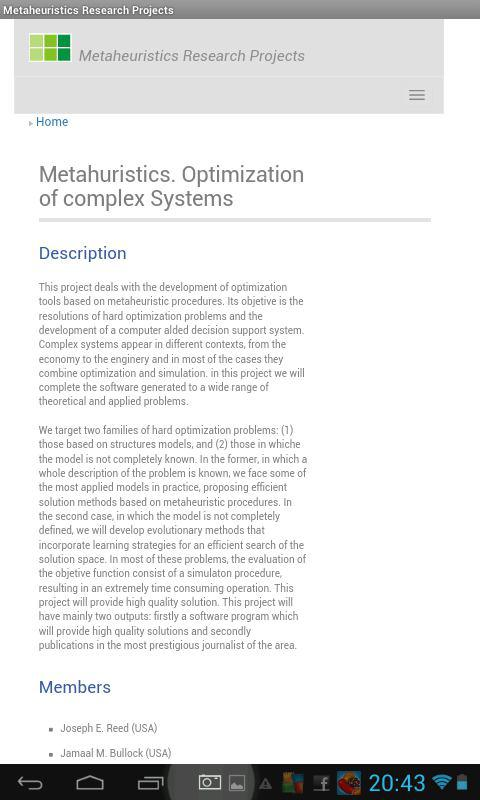
\includegraphics[width=65mm]{./imagenes/tablet}}
\caption{Diseño responsable de \texttt{index\_bootstrap.html}} \label{fig:responsible}
\end{figure}


\end{document}
